\documentclass[12pt, titlepage]{article}

\usepackage{booktabs}
\usepackage{tabularx}
\usepackage{hyperref}
\hypersetup{
    colorlinks,
    citecolor=black,
    filecolor=black,
    linkcolor=red,
    urlcolor=blue
}
\usepackage[round]{natbib}
\usepackage{graphicx}
\graphicspath{{./images/}}

%% Comments

\usepackage{color}

\newif\ifcomments\commentstrue %displays comments
%\newif\ifcomments\commentsfalse %so that comments do not display

\ifcomments
\newcommand{\authornote}[3]{\textcolor{#1}{[#3 ---#2]}}
\newcommand{\todo}[1]{\textcolor{red}{[TODO: #1]}}
\else
\newcommand{\authornote}[3]{}
\newcommand{\todo}[1]{}
\fi

\newcommand{\wss}[1]{\authornote{blue}{SS}{#1}} 
\newcommand{\plt}[1]{\authornote{magenta}{TPLT}{#1}} %For explanation of the template
\newcommand{\an}[1]{\authornote{cyan}{Author}{#1}}

%% Common Parts

\newcommand{\progname}{ProgName} % PUT YOUR PROGRAM NAME HERE
\newcommand{\authname}{Team \#, Team Name
\\ Student 1 name
\\ Student 2 name
\\ Student 3 name
\\ Student 4 name} % AUTHOR NAMES                  

\usepackage{hyperref}
    \hypersetup{colorlinks=true, linkcolor=blue, citecolor=blue, filecolor=blue,
                urlcolor=blue, unicode=false}
    \urlstyle{same}
                                


\begin{document}

\title{Verification and Validation Report: ESF} 
\author{Alaap Grandhi}
\date{\today}
	
\maketitle

\pagenumbering{roman}

\section{Revision History}

\begin{tabularx}{\textwidth}{p{3cm}p{2cm}X}
\toprule {\bf Date} & {\bf Version} & {\bf Notes}\\
\midrule
April 22 & 1.0 & Initial Version\\
\bottomrule
\end{tabularx}

~\newpage

% \section{Symbols, Abbreviations and Acronyms}

% \renewcommand{\arraystretch}{1.2}
% \begin{tabular}{l l} 
%   \toprule		
%   \textbf{symbol} & \textbf{description}\\
%   \midrule 
%   T & Test\\
%   \bottomrule
% \end{tabular}\\

% \wss{symbols, abbreviations or acronyms -- you can reference the SRS tables if needed}

\newpage

\tableofcontents

% \listoftables %if appropriate

% \listoffigures %if appropriate

\newpage

\pagenumbering{arabic}

This document ...

\section{Functional Requirements Evaluation}

For the System Functional Requirement tests, the input format testing process did not go as expected.
Specifically, I underestimated the amount of work that would need to go into processing the input images and pointclouds.
Converting input images and pointclouds into a unified format was relatively straightforward (load from the respective format into a numpy array and then convert that numpy array to a torch tensor), 
but I neglected the fact that the data processing pipeline contained quite a few steps. Even though I could load the images and pointclouds and then pass them through the respective feature encoders 
(straight into the model for the images and through a voxel encoder for the pointclouds), the fusion based approach here required also providing information on the local transformation matrices between 
the different sensors. Normally this would just mean that I would have to extract the sensor calibration parameters from the source dataset (nuscenes), but in this case nuscenes obscures these parameters 
behind their nuscenes-devkit API. Thus, I was not able to fully figure them out before the deadline and will add these tests into a future revision of the code and inference pipeline. At present, I decided to 
modify the code to simply visualize on NuScenes evaluation data directly collected from the NuScenes dataset itself (rather than on manually passed-in data). This will be fixed in a future revision over the next couple of days though.

For a similar reason, I instead changed my test-viz-correct procedure for now to a manual check. Rather than comparing to an already saved data visualization, I decided to visually inspect a few of the visualized 3D plots themselves. 
This is because comparing against data obtained from the dataset itself would not really work (since the eval dataset and corresponding loader are too big to be loaded automatically by github after trying). In the future, I will hand-pick a pointcloud and some 
images beforehand so that it does not require loading of the full dataset and can be run automatically by Github. For now, the resulting visualizations seemed correct and in-line with the visualizations NuScenes has \href{https://www.nuscenes.org/nuscenes}{on their website}.

Model consistency testing was deferred to a later date because I have yet to fully design an architecture that seems to work end-to-end (I am still facing a few bugs in a local version with the equivariant layer math). This will be added over the coming week though.


\section{Nonfunctional Requirements Evaluation}



\subsection{Accuracy}

Similarly to the model consistency testing suite, this test will be deferred to a later date due to issues in the equivariant layer module. This will also be coming over the next week.
		
\subsection{Understandability}

While I have not yet run through my questions and checklist with Dr. Matthew Giamou or my Domain Expert yet, I did do this with a lab member. Generally, they understood how the code worked at a high level,
 but had issues describing exactly what the submodules do due to the extensive nature of the code (the hour I spent discussing the code with them was not enough to get into the nuance of how the voxel feature encoder and bounding box losses work for example). 
They mentioned that at present, the documentation in the repository is lacking and that I would have to add more documentation in order for it properly explain how the code works. As such, I plan on adding an updated markdown file over the next few days to make 
the code more readable on its own. Since tasks like training and evaluation were high-level, they were able to perform them without assistance after the demo, but they struggled a bit with finding the exact configuration file to modify (the third task). I think that 
this is another sign that I need to add more extensive documentation to the code itself. Until this documentation is added, I would consider this test a fail for now.

\subsection{Installability}

Since I added scripts for installing the necessary requirements (in setup.sh) and for getting the pretrained models (in get\_models.sh), the installability aspect of the code was not too bad. The dataset setup guide (step 4) was skipped due to a lack of time for downloading the 
dataset but when I asked my lab member, they mentioned that it seemed fairly straightforward based on OpenPCDet's existing instructions. Since they did not install the dataset, I gave them access to a session on my home server to see if they could evaluate the pretrained model. 
This proceeded without any issues, so I would consider this test to be passed for now.

\subsection{Performance}

In training, each scene/frame was observed to take 35 seconds on average. While this is fairly slow, it is to be expected for training due to the computationally intensive backpropagation step. In inference, 7 scenes/frames on average were 
processed per second. This is much faster than the training speed, but is still much slower than the data capture rate of 30 frames per second. This indicates that more experiments should be done with models with fewer parameters (as to try to match the 30 fps capture rate).
	
\section{Comparison to Existing Implementation}	

This section will be filled in once the equivariant architecture is up and running.

\section{Unit Testing}

\subsection{Training Module Testing}

While training module testing cannot be conducted on an equivariant architecture yet (as it is not up and running at the moment), I did conduct the test for the existing 
BEVFusion architecture (\cite{liang2022bevfusion}). This was done to at least prove that the bounding box loss function was being optimized for the base pipelines (and that it in turn is being optimized for the equivariant architecture as the loss function remains unchanged). 
I still plan on replacing these results with ones for the equivariant architecture as soon as possible (over the next week). Overall, the training loss graph in figure \ref{Fig:Loss} (after training for 1 epoch which took 12 hours) shows a generally decreasing graph that does indeed confirm that the bounding box loss is being correctly minimized for the training dataset.

\begin{figure}[h]
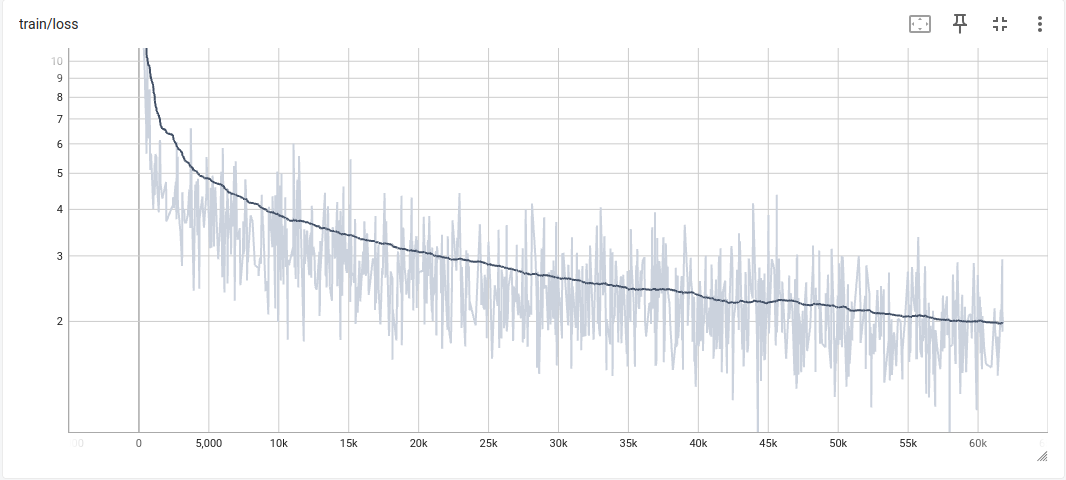
\includegraphics[width=15cm]{loss}
\caption{A plot showing the bounding box loss (on the y-axis) against the number of batches trained on (on the x-axis)}
\label{Fig:Loss}  
\end{figure}


\subsection{Evaluation, Checkpoint, Config, and Data Module Testing}

After evaluating the pretrained NuScenes BEVFusion model, I have confirmed that the results do match those presented on the OpenPCDet Github. I have added a table comparing the two below. 
Note that here mATE represents mean translation error, mASE represents mean scale error, mAOE represents mean orientation error, mAVE represents mean velocity error, mAAE represents mean attribute error, mAP represents 
mean average precision, and NDS represents a NuScenes specific evaluation metric. Since it is the most commonly cited metric in the literature, the mAP metric is what I am using for evaluation but 
the remaining metrics are still also reported to ensure consistency between them as well. 
\newline


\begin{tabular}{lccccccccl}\toprule
  & mATE & mASE & mAOE & mAVE & mAAE & mAP & NDS \\\midrule
  OpenPCDet Results & 28.03 & 25.43 & 30.19 & 26.76 & 18.48 & 67.75 & 70.98 \\
  \addlinespace
  Local Results & 28.05 & 25.44 & 30.18 & 26.79 & 18.45 & 67.76 & 70.99 \\
  \bottomrule
\end{tabular}

\subsection{Equivariant Layers Module Testing}

This section will be filled in once the equivariant architecture is up and running.

\section{Automated Testing}

This section will be filled in once the aforementioned issues with automated data loading are fixed.

\subsection{Inference Module Testing}

% \section{Trace to Requirements}
		
% \section{Trace to Modules}		

% \section{Code Coverage Metrics}


\bibliographystyle{plainnat}
\bibliography{../../refs/References}

\newpage{}

\end{document}